\documentclass[border=5mm]{standalone}
\usepackage{tikz}
\usetikzlibrary{arrows.meta}

\definecolor{darkblue}{rgb}{0.1, 0.2, 0.6}
\definecolor{darkgreen}{rgb}{0.1, 0.5, 0.1}

\begin{document}

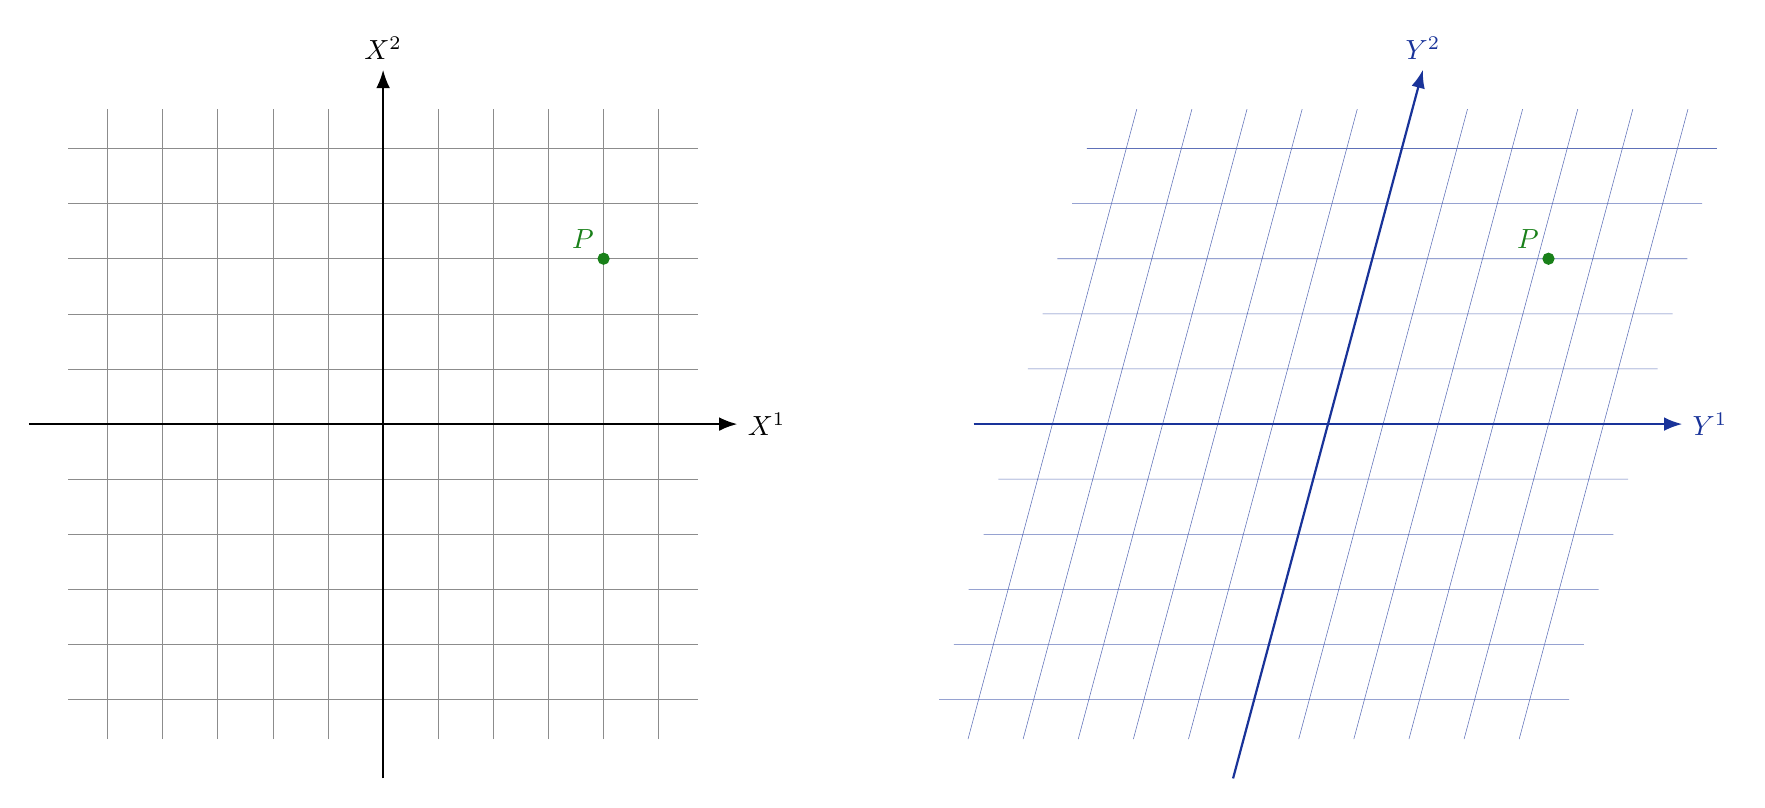
\begin{tikzpicture}
    \tikzstyle{axis_style} = [-Latex, thick, black]
    \tikzstyle{y_axis_style} = [-Latex, thick, darkblue]
    
    \def\px{4*0.7}
    \def\py{3*0.7}
    
    \begin{scope}
    	\draw[step=0.7cm, color=gray!90, very thin] (-4,-4) grid (4,4);
  	  \draw[axis_style] (-4.5,0) -- (4.5,0) node[right] {$X^1$};
   	  \draw[axis_style] (0,-4.5) -- (0,4.5) node[above] {$X^2$};
	    \filldraw[darkgreen] (\px,\py) circle (2pt) node[above left] {$P$};
    \end{scope}
    
    \begin{scope} [xshift=12cm, xslant=tan(15)]
      \draw[step=0.7cm, color=darkblue!70, very thin] (-4,-4) grid (4,4);
      \draw[y_axis_style] (-4.5,0) -- (4.5,0) node[right] {$Y^1$};
	    \draw[y_axis_style] (0,-4.5) -- (0,4.5) node[above] {$Y^2$};
    \end{scope}
    
    \begin{scope}[xshift=12cm]
        \filldraw[darkgreen] (\px,\py) circle (2pt) node[above left] {$P$};
    \end{scope}
    
\end{tikzpicture}
\end{document}
